\section{Estimating Relative Orientations from Projections}
\label{sec:estimating-relative-orientations}

Equipped with the geodesic distance $d_q$, our goal is now to find a ``projection distance'' $d_b$ that is a good predictor of $d_q$. Before discussing the different options, we briefly describe the synthetic datasets used in this work.  

% -------------------------------
\subsection{Experimental Dataset}
\label{subsec:datasets}

We consider two proteins as ground truths: the $\beta$-galactosidase, a protein with a dihedral (D2) symmetry, and the lambda excision HJ intermediate (HJI), an asymmetric protein. Their deposited PDB atomic models are 5a5a ~\cite{bartesaghi2015betagal} and 5j0n~\cite{laxmikanthan2016structure}, respectively. For each atomic model, we generate the ground truth by fitting a 5\AA\ density map in Chimera~\cite{pettersen2004ucsf}. We thus obtain a volume of size $(117\times 117\times 117)$ for the $\beta$-galactosidase, and a volume of size $(275\times 275\times 275)$ for the HJI.  

From these ground truths, we generate $5,000$ synthetic projections of size $(117\times 117)$ and $(275\times 275)$, respectively, using the ASTRA projector~\cite{van2015astra}. The projection orientations are sampled from a uniform distribution over half the $\SOThree$ space, which suffices to generate all the possible projections of a volume. For the sake of simplicity, the projections are currently kept unblurred and noiseless. Whenever training neural networks, we split the datasets into a distinct training set (50\%), validation set (22\%), and testing set (33\%), to ensure that the results can generalize to unseen projections. The complete pipeline is implemented in Tensorflow~\cite{abadi2016tensorflow}. 


% -------------------------------
\subsection{Baseline Test with the Euclidean Distance}

As a baseline, we first evaluate the suitability of the Euclidean distance as a projection distance $d_b$ to predict $d_q$. For the two aforementioned datasets, we randomly select $1,000$ pairs of projections. For each pair, we compute the Euclidean distance between the projections $d_b(\mathbf{b}^i,\mathbf{b}^j)=\lVert\mathbf{b}^i-\mathbf{b}^j\rVert_2$ and their relative orientation $d_p(q_i,q_j)$ through~\eqref{eq:geodesic distance}. We then report the $(d_q,d_b)$ relationship for all pairs in Figure~\ref{fig:euclidean-not-robust}, for both the asymmetric protein (left) and the symmetric one (right). 


Two principal observations can be made from this experiment. First, as suspected, the Euclidean distance between projections fails to be a consistent predictor of their relative orientation distance, even in the simple imaging conditions considered here (no noise and no effect of the PSF). In particular, the larger the relative distance $d_q$, the poorer the predictive ability of the Euclidean distance as $d_b$. The other interesting observation is that the intrinsic symmetry of the $\beta$-galactosidase protein (5a1a) appears in its $(d_q,d_b)$ plot.

%-----
\begin{figure}[t]
    \centering
    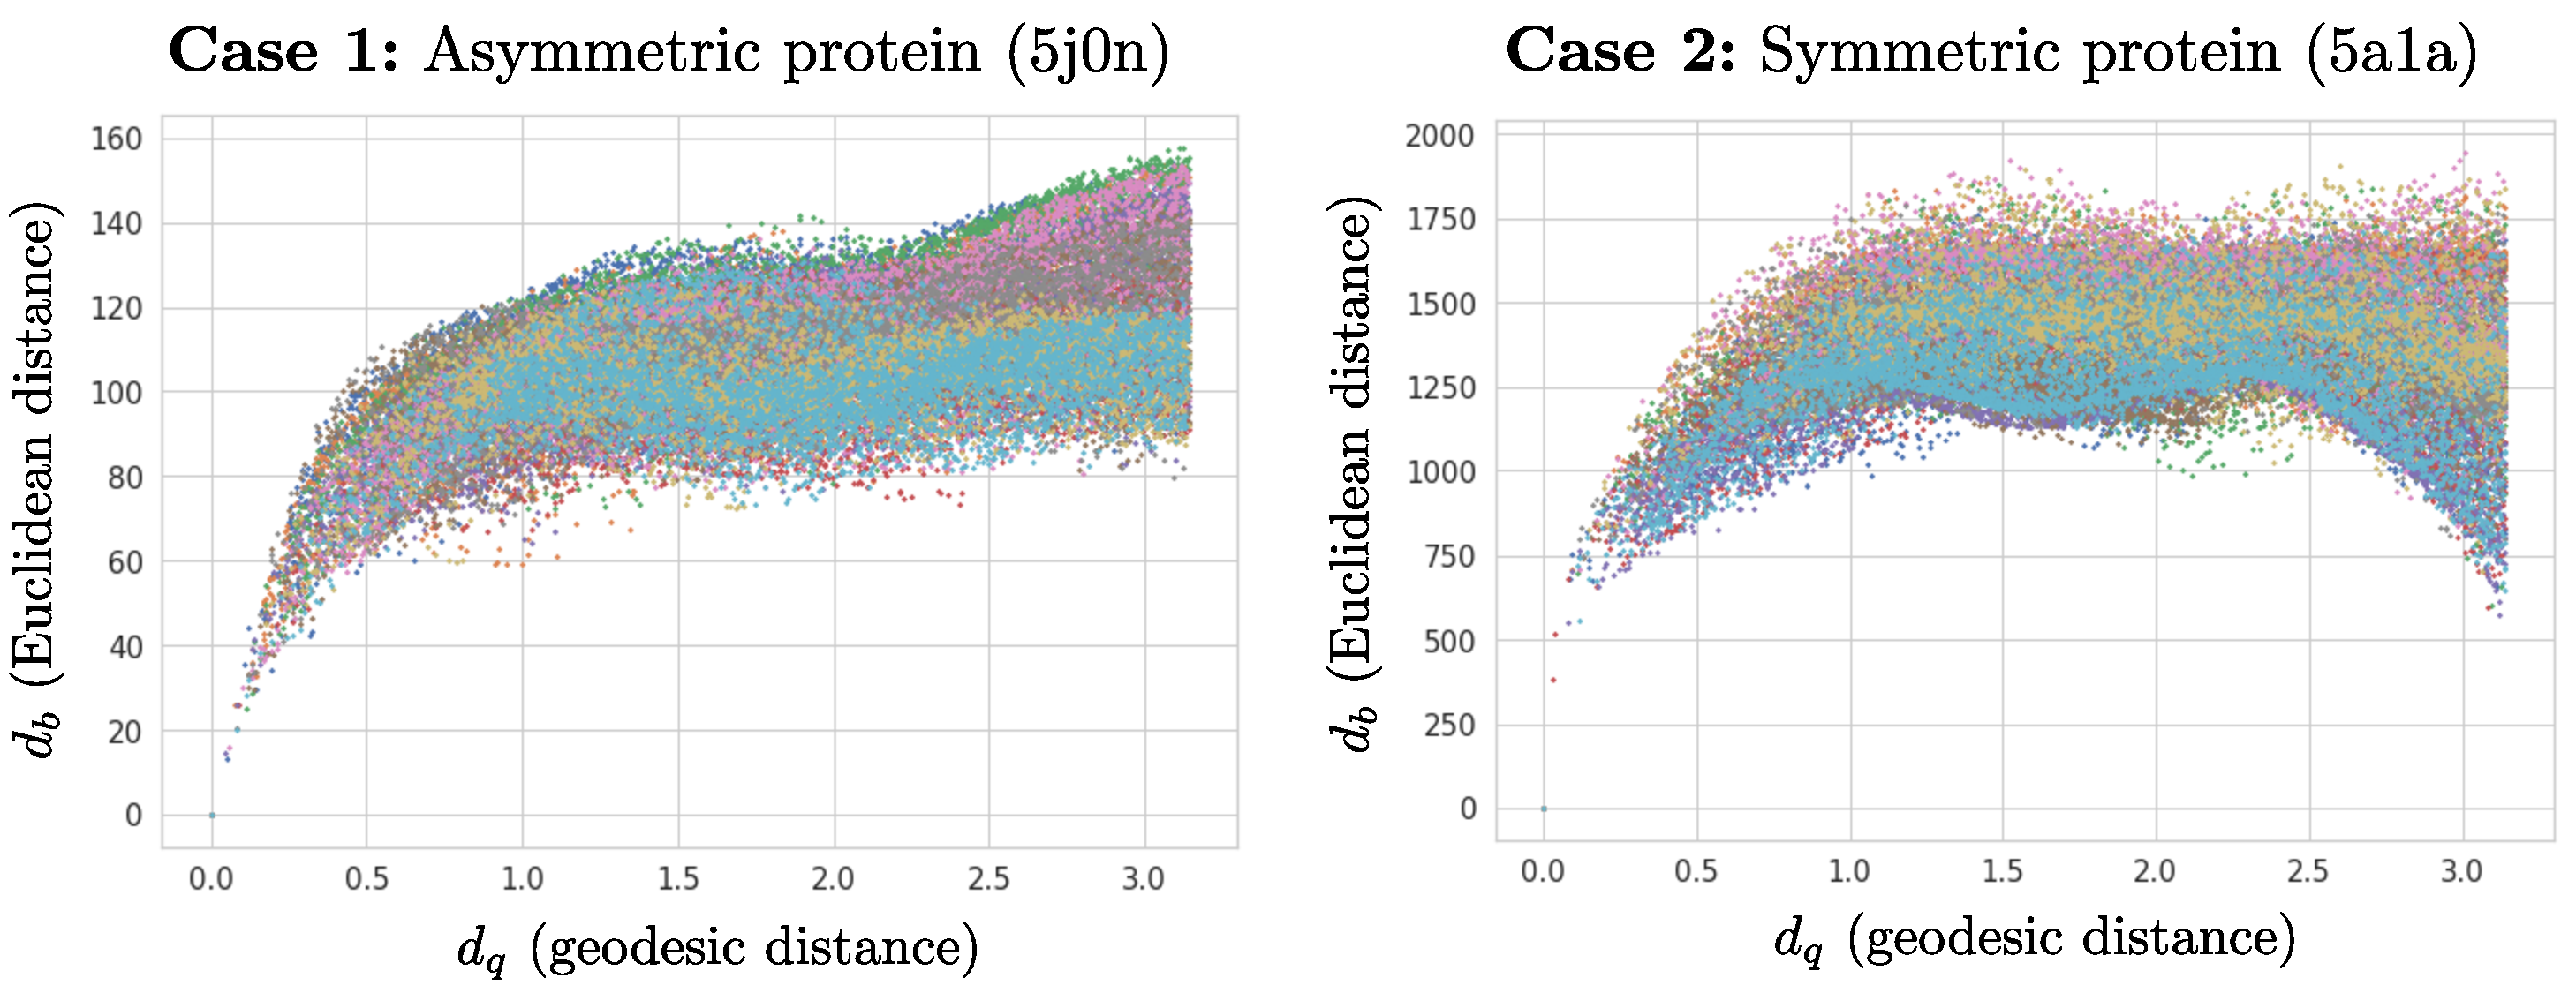
\includegraphics[width=\textwidth]{EuclideanDistance_NonRobust.pdf}
    \caption{Plotting the Euclidean distance between two projections versus their actual relative orientation (measured by the geodesic distance) for \textbf{(left)} the asymmetric protein (5j0n) dataset, and \textbf{(right)} the symmetric protein (5a1a) dataset. }
    \label{fig:euclidean-not-robust}
\end{figure}
%---- 

% -------------------------------
\subsection{Learning $\widehat{d}_b$ with a Siamese Neural Network}

As previously discussed, we make the choice to \textit{learn} a good approximation $\widehat{d}$ on a synthetic training dataset $\big\{ \mathbf{b}^{*p}, q^*_p\big\}_{p=1}^{N_t}$ through 
%---
\begin{equation}
    \label{eq:metric-learning-siamese}
    \widehat{d}_b=\argmin{d_b}\sum_{i,j} \big|d_b\big(\mathbf{b}^{*i},\mathbf{b}^{*j}\big) - d_q\big(q^*_i,q^*_j\big) \big|^2, 
\end{equation}
% --- 
with $d_q$ defined in~\eqref{eq:geodesic distance}, and where $N_t$ indicates the number of projection-orientation pairs in the training dataset. More precisely, we parametrize the distance function $d_b$ in~\eqref{eq:metric-learning-siamese} as a Siamese neural network (SiameseNN)~\cite{chopra2005learning}, and resort to learning its weights $w$, as illustrated in Figure~\ref{fig:siamese-schematic}. 

SiameseNNs, also termed ``twin networks'', are commonly used in the field of deep metric learning to learn similarity functions~\cite{yi2014deep}. They are usually constituted of two sister neural networks that work in tandem and share the exact same architecture and weights.  Their role (once trained) is to extract the projection features that are the most relevant to predict the relative orientation between two projections. The weights $w$ of the two sister networks are progressively learned by 1) comparing the difference of their projection feature vectors to the magnitude of the corresponding relative orientations, and 2) back-propagating this error (via the derivative chain rule) to the weights. 

%---
\begin{figure}[t!]
    \centering
   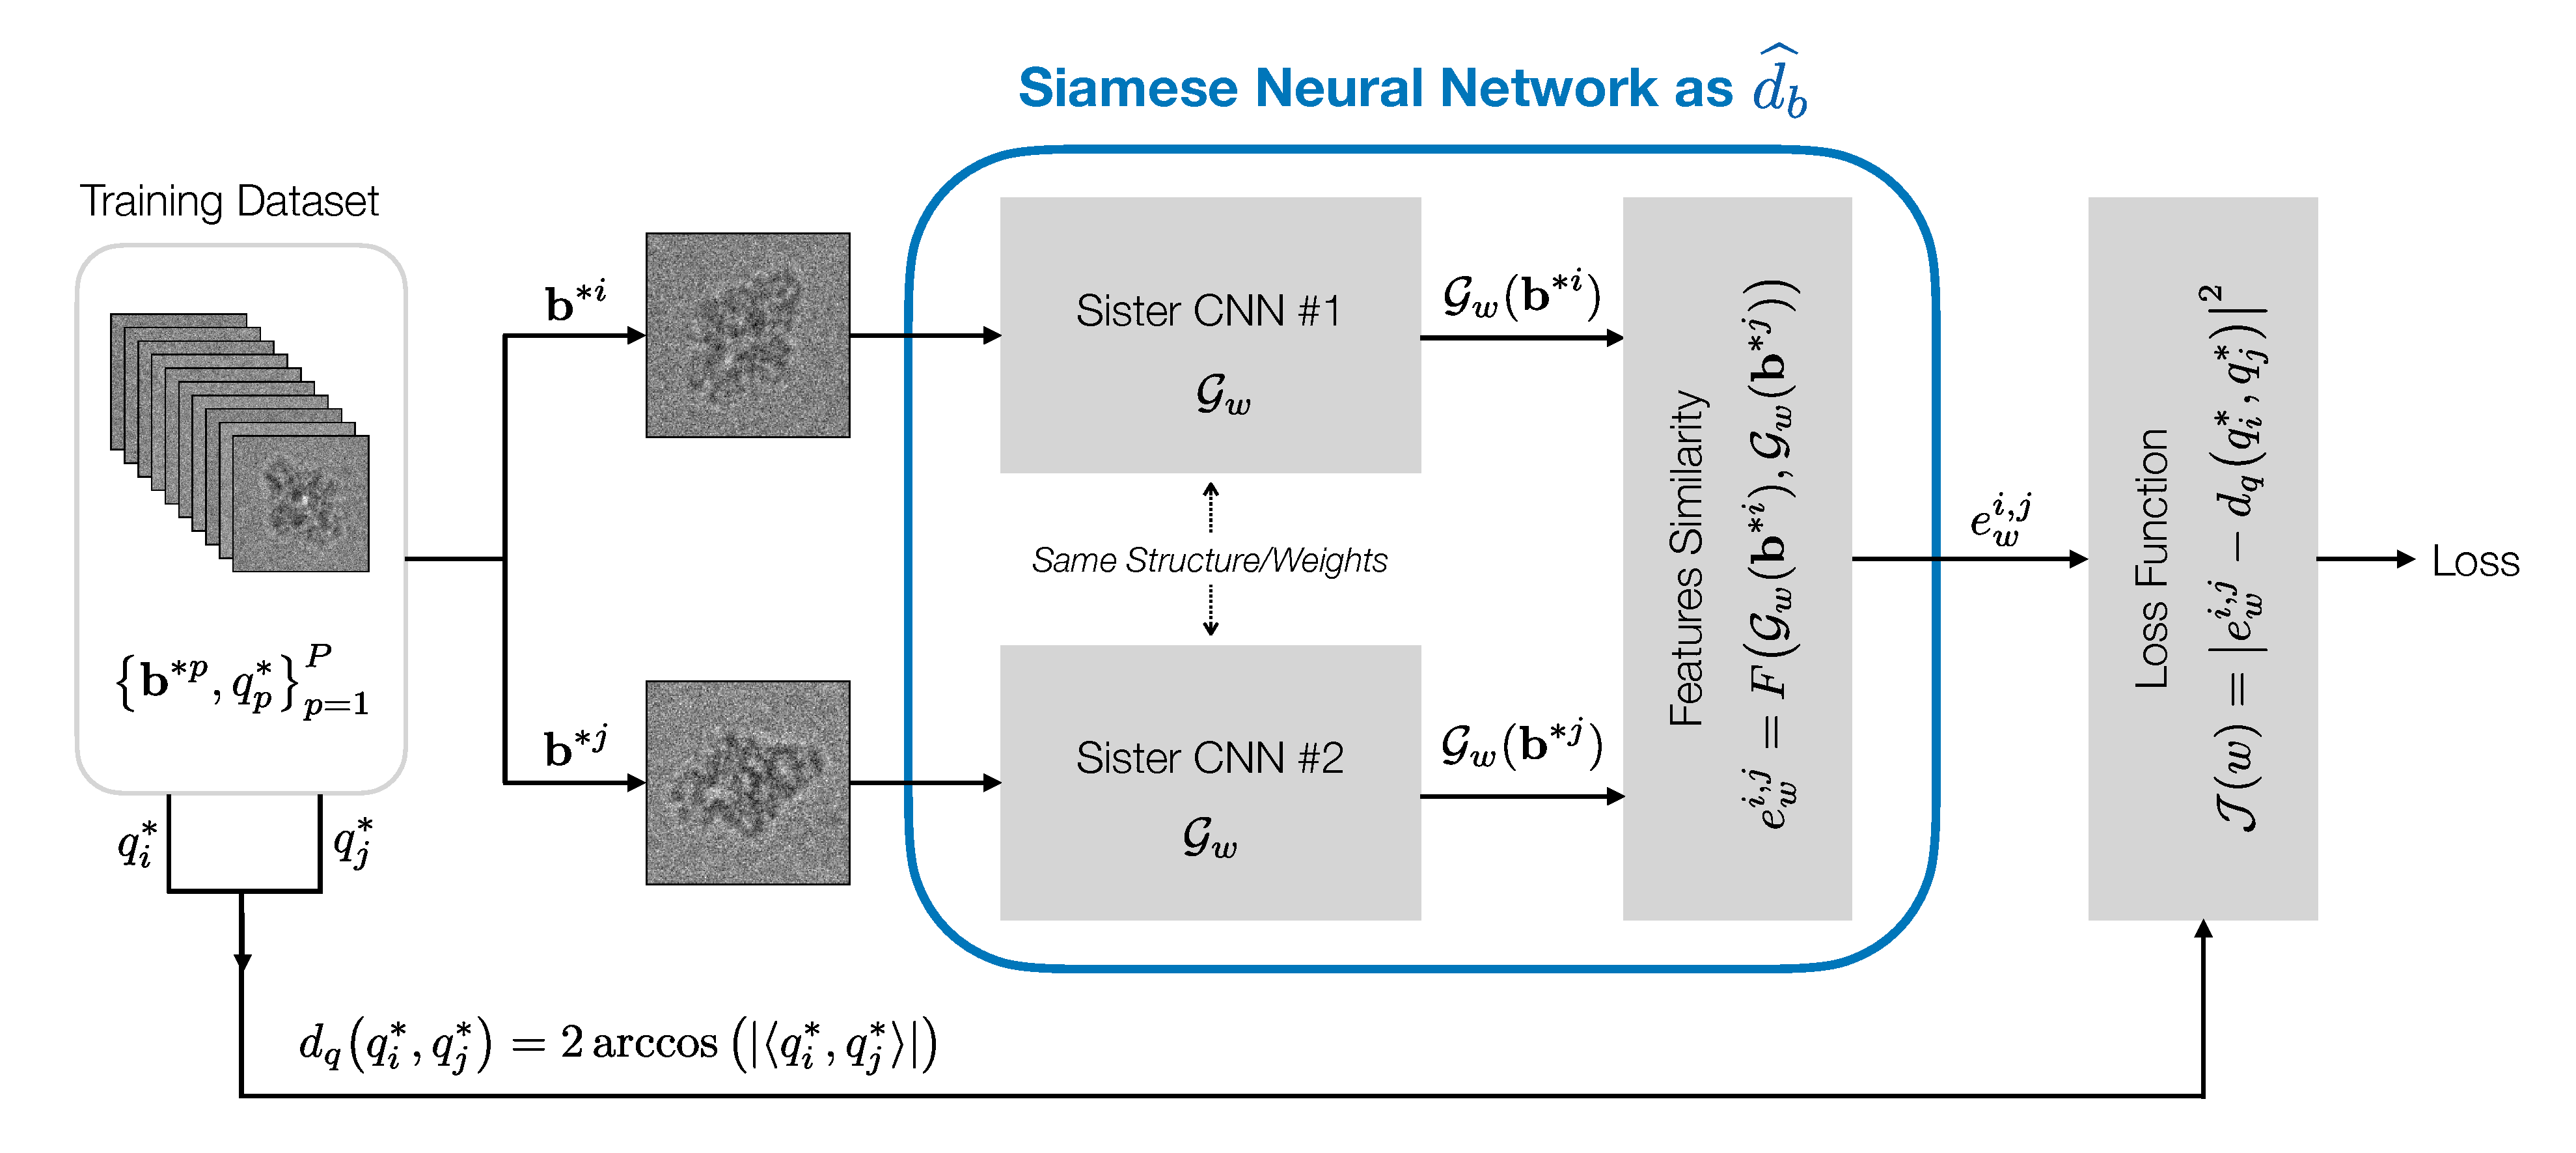
\includegraphics[width=\textwidth]{siameseNN-schematic.pdf}
    \caption{Training a Siamese neural network (SiameseNN) to become a faithful predictor of the relative orientation between two input projections. In other words, we train the SiameseNN to serve as a projection distance $\widehat{d}_b$ that correctly approximates the orientation distance $d_q$. The training is performed with a synthetic dataset that contains thousands of projections with their associated orientation.}
    \label{fig:siamese-schematic}
\end{figure}
% --- 

% ----------------------------------------------------
\subsubsection{Generating a Proper Training Dataset for the SiameseNN}
\label{sec:training-siamese}

The success of the SiameseNN as a faithful predictor of relative orientations eventually relies on our capacity to generate a synthetic training dataset that is both large and representative of SPA measurements. In other words, we need to create a training set whose data distribution is diverse enough to cover that of unseen projection datasets. The objective is for the SiameseNN to be able to handle projections acquired in all sorts of imaging conditions and originating from 3D volumes it has never been trained on. 

We shall create such comprehensive training dataset by capitalizing on two favorable conditions. First, there exists a large publicly-available database of deposited atomic models of proteins, which gives us access to thousands of different 3D ground truths. Then, we shall take advantage of our ability to model the cryo-EM imaging procedure to generate, from these ground truths, a synthetic dataset that contains a massive amount of realistic projections whose orientations are, by definition, all known. 

Note that an interesting aspect of SiameseNNs for the present application is that they intrinsically predict the \textit{relationship} between objects. Hence, a well-trained SiameseNN could be relatively robust to the change of volumes. In the same line of thought, our SiameseNN will likely benefit from the profound structural similarity shared by proteins---after all, they all derived from just the same 21 amino acids.  


% ----
\begin{figure}[t!]
    \centering
    \begin{subfigure}[t]{0.4\textwidth}
        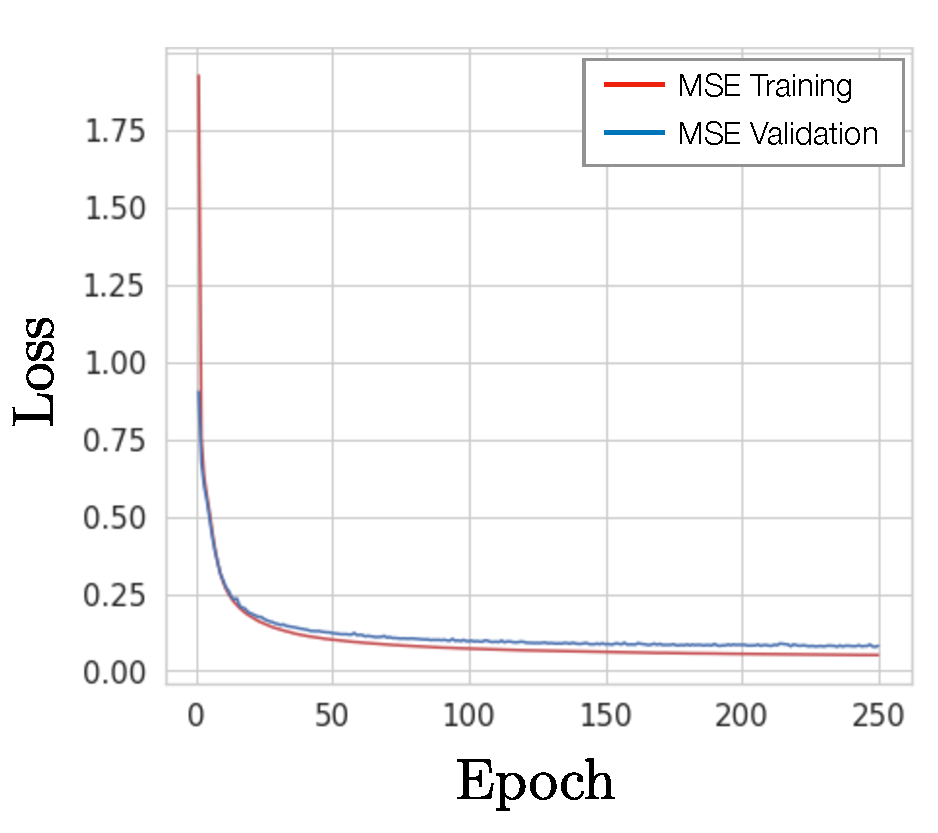
\includegraphics[width=0.98\textwidth]{TrainingSiamese_LossAssymetric.pdf}
        \caption{Training losses of the SiameseNN on the asymmetric protein (5j0n) training and validation datasets.} 
        \label{fig:losses-siamese-assym}
    \end{subfigure} \quad \quad
    %
    \begin{subfigure}[t]{0.4\textwidth}
        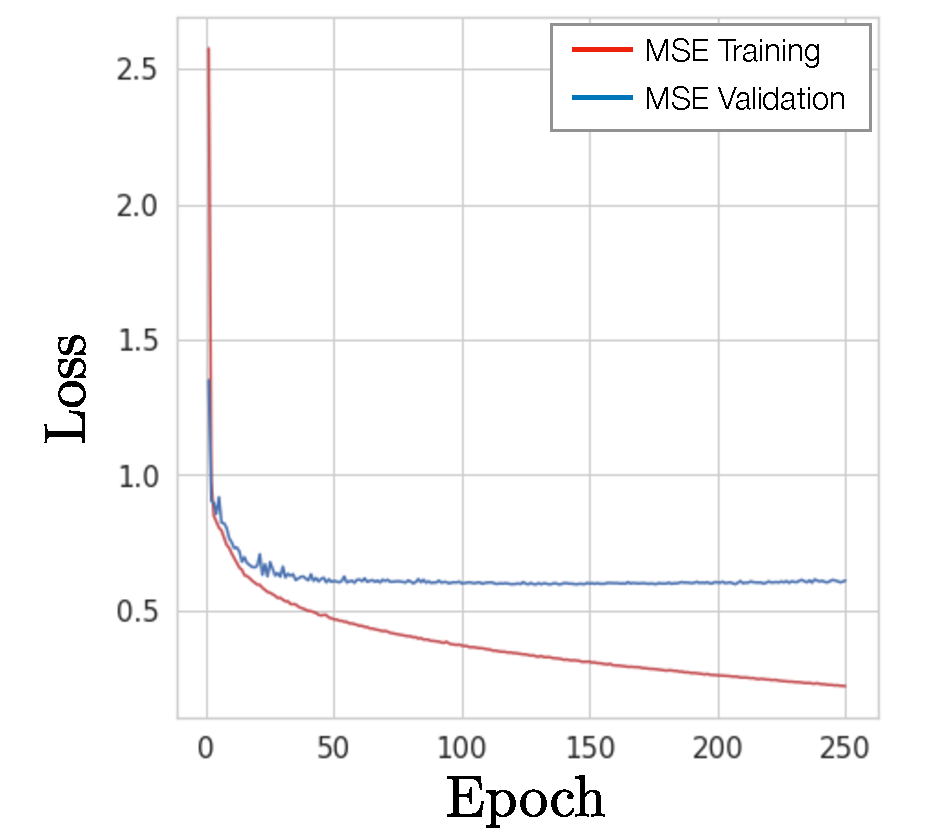
\includegraphics[width=0.98\textwidth]{TrainingSiamese_LossSymetric.pdf}
        \caption{Training losses of the SiameseNN on the symmetric protein (5a1a) training and validation datasets.} 
        \label{fig:losses-siamese-sym}
    \end{subfigure} \vspace{0.45cm}
    
    %
    \begin{subfigure}[t]{0.4\textwidth}
        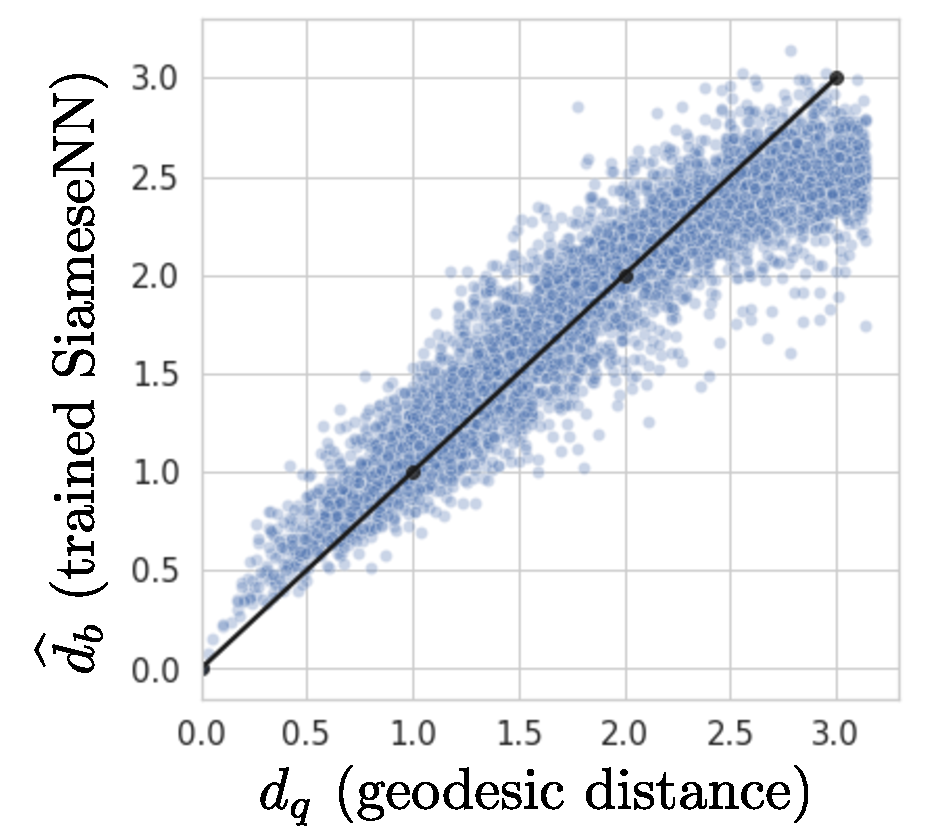
\includegraphics[width=0.98\textwidth]{TrainingSiamese_PlotAssymetric.pdf}
        \caption{Relative orientations predicted by the trained SiameseNN from projections in the asymmetric protein (5j0n) testing dataset. } 
        \label{fig:learned-distance-siamese}
    \end{subfigure} \vspace{0.35cm}
    \caption{Training results for the SiameseNN.} 
    \label{fig:losses-siamese}
\end{figure}
% ---


% ----------------------------------------------------
\subsubsection{Preliminary Training Results}

We present here a preliminary evaluation of the ability of SiameseNNs to learn a projection distance $\widehat{d}_b$ that correctly approximates the orientation distance $d_q$. 

SiameseNNs come with a variety of more or less powerful architectures. At the current stage of development, we work with a simple one. Our SiameseNN is composed of two convolutional neural networks (CNNs) with shared weights. Their output features vectors are compared through an Eulidean distance, \textit{i.e.}, $F(\mathbf{x},\mathbf{y})=\lVert \mathbf{x}-\mathbf{y}\rVert_2$ in Figure~\ref{fig:siamese-schematic}. The detailed architecture of this SiameseNN is given in Figure~\ref{fig:app-SiameseNN-architecture} in Appendix X.

For each protein, we train the SiameseNN on its training dataset for 250 epochs ($\sim$10 hours) using an Adam optimizer~\cite{kingma2014adam}, a learning rate of $10^{-3}$, and a batch size of 256 projections. The evolution of the training and validation losses are presented in Figure~\ref{fig:losses-siamese-assym} for the asymmetric protein (5j0n), and in Figure~\ref{fig:losses-siamese-sym} for the symmetric one (5a1a). The results demonstrate that the SiameseNN succeeds at learning a proxy distance for the asymmetric protein dataset, as convergence is reached in about 50 epochs ($\sim$ 2 hours). 

However, the current SiameseNN architecture fails at learning the distance for the dataset 5a1a, which is very likely due to the symmetry of the $\beta$-galactosidase protein. Indeed, its synthetic dataset contains pairs of projections that share the same $d_b$, yet differ in their $d_q$. This simply advocates for the restriction to non-overlapping areas on $\SOThree$ when sampling the orientations used to generate the SiameseNN training dataset. The latter would then only contain projection pairs with a linear $(d_q,d_b)$ relationship, which should ensure a successful training of the network. For the rest of the experiments, we use the asymmetric protein (5j0n) dataset. 

We then feed to the trained SiameseNN $1,000$ pairs of projections randomly selected from the 5j0n testing dataset, and report the $(d_q,\widehat{d}_b)$ relationship of each pair in Figure~\ref{fig:learned-distance-siamese}. These results confirm that, for this protein at least, the SiameseNN is able to predict the orientation distance $d_q$ using only the projections as inputs. Moreover, it clearly outperforms the Euclidean distance at doing so. These preliminary results are encouraging, as much has yet to be gained from improving upon the rather primitive SiameseNN architecture we currently use.